\section{EXPERIMENTS AND EVALUATION}
\label{sec:exper}
\begin{figure*}[!th]
	\centering
	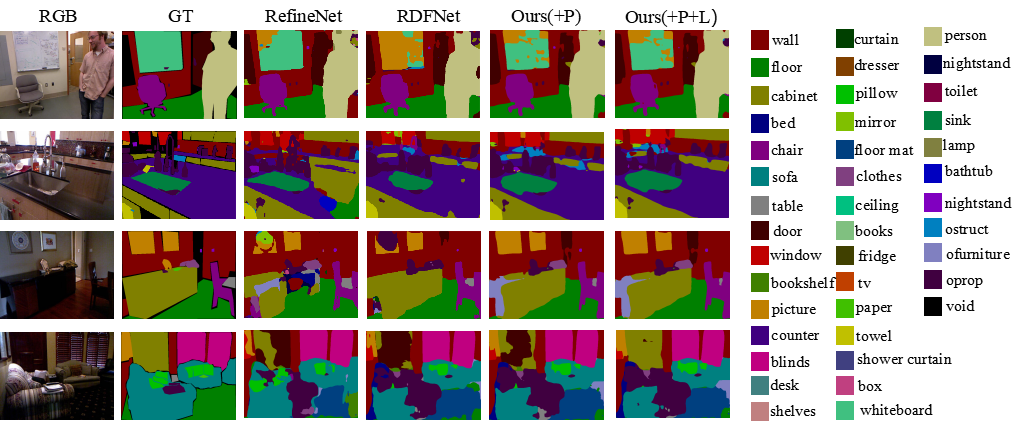
\includegraphics[scale=0.6]{figure/Result.png}
	\caption{Qualitative results on the NYUD—v2 dataset. For the secne image in each row, we show: the RGB image; the ground truth of semantic segmentation; the result of RefineNet; the result of RDFNet; the result of trained by $L_{Consistency}$; the result of trained by $L_{PGT}$ and the result of trained by two losses. Our method predicts more accurate and complete segmentation results.}
	\label{fig:VisResult}
\end{figure*}
To demonstrate the validity of proposed appoaches for indoor scene segmentation, we conduct the experiments on a publicly available benchmark dataset (NYUD-v2) which provides many sequences of RGBD data. 
%
The performance is presented to show the benefits of our methods.
%
In the following we describle the details of our evaluation results.


{\bf{Dataset and Evaluation Metrics.}} 
The NYU Depth v2 dataset includes many RGB-D sequences of 464 indoor scenes captured from a Kinect sensor. 
%
It just consists of 1449 annotated images, 795 of them are used for training and the remaining 654 images for testing.
%
In our experiment, we map the semantic labels into 40 categories, according to \cite{Gupta2014}.
%
The training data are augmented during the training phase. 
%
We perform data augmentation on the training RGB and HHA images by random horizontal flips with a possibility of 0.5, scaling the images with a selected ratio in $\left\{0.7,0.8,0.9,1.0,1.2,1.3\right\}$ and random cropping. 
%
All our experiments are conducted on a single Nvidia Titan X Pascal GPU, using the Caffe framework.


Following previous works
\cite{Eigen2015,Gupta2014,Kendall2015,Lin2016,Lin2017,Li2016,Cheng2017,Park2017,Xu2018,Zhang2018,Jiao2018}, we use several quantitative metrics to evaluate our semantic segmentation results, including pixel 
accuracy, mean accuracy and mean IOU. 
%
\begin{table}[!htbp]
	\vspace{-0.4cm}
	\centering
	\caption{Comparsions of different network architectures on NYU v2 Dataset.}
	\begin{tabular*}{8.7cm}{lllll}
		\hline
		Method & data & pixel acc. & mean acc. & IoU\\
		\hline \hline
		B-SegNet \cite{Kendall2015} & RGB &68.0 & 45.8 & 32.4 \\
		Context \cite{Lin2016} & RGB & 70.0 & 53.6 & 40.6 \\
		RefineNet \cite{Lin2017} & RGB & 73.6 & 58.9 & 46.5\\
		\hline
		Gupta et al. \cite{Gupta2014} & RGBD & -- & 35.1 &--\\
		Eigen et al. \cite{Eigen2015} & RGBD & 65.6 & 45.1 & 34.1\\
		FCN \cite{Long2015} & RGBD & 65.4 & 46.1 & 34.0 \\
		LSTM-CF \cite{Li2016} & RGBD & --& 49.4 & -- \\
		Cheng et al.\cite{Cheng2017} & RGBD & 71.9 & 60.7 & 45.9 \\
		RDFNet \cite{Park2017} & RGBD & 76.0 & 62.8 & 50.1\\	
		\hline
		baseline &RGBD & 75.8 & 63.0 & 50.0\\
		Ours(+$L_C$) & RGBD & 75.8 & 63.3 & 50.1\\
		Ours(+$L_{P}$) & RGBD & 75.9 & 63.6 & 50.2\\
		Ours(+$L_{C}$+$L_{P}$)& RGBD & 75.8 & \bf{63.8} & 50.2\\
		\hline
		PAD-Net \cite{Xu2018} & RGB &75.2 & 62.3 & 50.2\\
		TRL \cite{Zhang2018} & RGB &76.2 & 56.3 & 46.4\\
		Jiao et al.\cite{Jiao2018} & RGB & \bf{81.1} & 62.2 & \bf{50.9}\\
		\hline		 		
	\end{tabular*}
	\label{Tab:Results}
\end{table}
%
Let $m_{kj}$ denote the number of pixels of class ${k}$ classified as class ${j}$.
%
Assuming the number of categories is $c$, $m_{k} = \sum_{j}m_{kj}$ is the total number of pixels belonging to class $k$. 
%
And $I = \sum_{k}m_{k}$ denotes the number of all pixels.
%
The three metrics are defined as follows:\\
\renewcommand{\baselinestretch}{1.0}\indent\text{---} pixel accuracy: $\sum_{k}m_{kk}/I$;\\
\indent\text{---} mean accuracy: $\frac{1}{c}\sum_{k}m_{kk}/m_{k}$;\\
\indent\text{---} mean IOU: $\frac{1}{c}\sum_{k}m_{kk}/(m_{k}+\sum_{j}m_{jk}-m_{kk})$ ;\\


{\bf PGT Analysis.} We present a example of the generated PGT in Fig.~\ref{fig:PGT}.
%
It can be seen that PGT contains noisy samples. 
%
But on the other hand, PGT can also be reliable enough.
%
We set the RDFNet as our baseline.
%
Because of the differences of hardware, we get the slightly different result from the official code.
%
The results on NYUD-v2 dataset are shown in Table~\ref{Tab:Results}.
%
As the table shows, although the PGT contains noisy labels, the performs of RDFNet still increase obviously. 
%
Especially in the mean accuracy.
%
and we achieve state-of-the-art performance on mean accuracy.
%
Compared to the baseline, our approach improves the pixel accuracy by more than 0.1\% as well as mean IOU by more than 0.2\%.
%
More quantitative results are shown in Fig.~\ref{fig:VisResult}.
%
To facilitate future researches, we will release our PGT dataset.

{\bf{Training Semantic Segmentation Network using Temporal Consistency Analysis.}} 
To discover the effectiveness of our proposed training policy. 
%
We conduct our experiments on generated PGT data with temporal consistency loss.
%
The quantitative and qualitative results are shown in Table~\ref{Tab:Results} and
Fig.~\ref{fig:VisResult} respectively.
%
To prove that performance improvements are not just due to PGT, we did an ablation study by removing $L_{PGT}$.
%
The results are shown in Table~\ref{Tab:Results} and Fig.~\ref{fig:VisResult}.
%
Compared to baseline, the mean accuracy and IOU are all been promoted.
%
Using $L_{consistency}$ and $L_{PGT}$ simultaneously, the mean accuracy is improved by 0.8\%.
%
And mean IoU is improved by 0.2\%.
%
And our method achieves the comparable performance as multi-task learning method.

{\bf{Dicussion.}} In the course of our experiment, we find the ground truth proposed by NYUD-v2 data set exits some annotation errors shown in Fig.~\ref{fig:mislabels}.

\begin{figure}[!htbp]
	\setlength{\abovecaptionskip}{-0.2cm}
	\setlength{\belowcaptionskip}{-10cm}
	\centering
	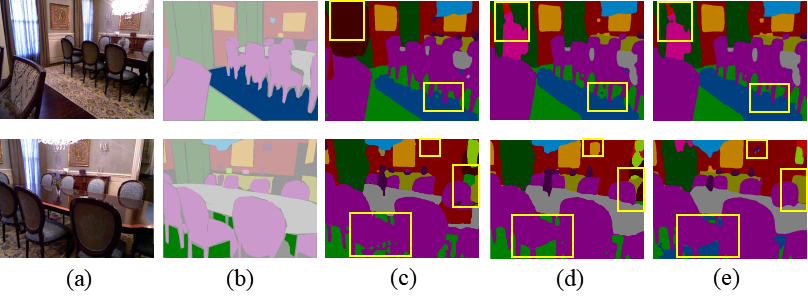
\includegraphics[scale=0.4]{figure/Mislabels.png}
	\caption{Mislabeled images. (a) is two frames of one scene provided by NYUD-v2 test set. (b) shows the corresponding labels of them. The mislabled pixels are highlighted. (c)(d)(e) are prediction results of RefineNet, RDFNet and our model. The details are framed in yellow.}
	\label{fig:mislabels}
\end{figure}
%
But our proposed method shows a more robust result compared to RefineNet \cite{Lin2017} and RDFNet \cite{Park2017}.
%
There are still some difficult classes in NYUD-v2 data set, such as bag and box.
%
The pixel accuracy and IOU is under 30\%.
%
The main reason is that the size of these two kinds of object is too small and the occurrence frequency of them is very low. 






